\chapter{Literature Review}

\paragraph{}
In this section we will give a review about theories and related work of this research. 

\section{Graphs in Real World}

\paragraph{}
Many real world datasets can be mapped into graphs. The users and the interactions between them, details about packet transfer in a computer network and a large citation database with authors of the research papers and their publications are some of the real world scenarios that could be mapped into graphs perfectly. Due to the sheer volume of the original datasets, the graphs produced from these datasets are also massive in size. 

\paragraph{}
Keeping these massive graphs in memory has become unrealistic with the large capacity that is required to store them. There are many challenges that lies in utilizing these graphs to derive knowledge through their properties while keeping them stored in secondary storage devices. This becomes easily evident in a scenario of a social network like Facebook or Twitter. Millions of user accounts interact with each other adding a large number of edges to the graph in a unit time. Retrieving the properties of this constantly evolving graph in realtime poses many difficulties. 

\paragraph{}
The properties of a graph that needs to be retrieved vary widely with the application scenario. In a social network it would be vital in finding the heavy hitter edges depicting the interaction between users or reachability of nodes showing how close the specific users are related. Model of a computer network would benefit with queries in finding heavy hitter nodes indicating possible destinations and sources of attacks originating within the network. Empirically, most real world graphs sparse and obey power law degree distribution. Most importantly, many of the real world scenarios get mapped into graph streams rather than static graphs. 

\section{Streaming Graphs}

\paragraph{}
Graphs can be divided into two as static graphs and streaming (dynamic) graphs. Static graphs are those which do not  change over time while streaming graphs are the ones which do get updated over time. These update operations could be insertion or deletion of nodes and edges. 

\paragraph{}
Determining the properties of streaming graphs is relatively strenuous than static graphs as they are constantly evolving. Usual graph algorithms cannot be run on streaming graphs due to their dynamic nature. Either the updating queries has to be stopped or a separate snapshot of the past should be used while running the graph algorithms. This is made even more difficult with the speed with which the graph is being updated. High throughput of update queries require any other types of queries to be run efficiently and as fast as possible in an unblocking manner. 

\paragraph{}
Real world streaming graphs could grow very large in size. Therefore these graphs are often stored as partitions in different machines over a network rather than in a single location. 

\section{Graph Partitioning}

\paragraph{}
The size of modern datasets has become too large to be fit into a single machine. It has become unrealistic to try to process the graphs mapped to these massive datasets while keeping them in the memory of a single node. Hence there exist a need to partition those large scale graphs into multiple machines. The communication between groups should be minimal to run graph algorithms on the whole graph effectively. However graph partitioning has been proved to be an NP-hard problem\cite{garey_simplified_1974}. Therefore the graph partitioning algorithms are only able to give sub-optimal solutions as of this date and thus a good streaming graph partitioning algorithm is impossible\cite{stanton_streaming_2012}. Graph partitioning algorithms can be mainly divided into two, such that, Online Graph Partitioning Algorithms and Offline Graph Partitioning Algorithms. The offline partitioning algorithms such as METIS\cite{karypis_fast_1998}, Chaco\cite{hendrickson_chaco_1993}, SBV-cut\cite{kim_sbv-cut:_2012} need to load the entire graph into the memory for the algorithm to be run. But the online partitioning algorithms like PreferBig\cite{stanton_streaming_2012} and HoVerCut\cite{sajjad_boosting_2016} keeps a buffer of the edge streams and process them when the buffer gets full. 

\section{Graph Summarization}

\paragraph{}
Reducing the complexity of a graph while retaining some of its original properties is known as graph summarization. These summaries often incur an error when running algorithms due to the loss of information. But usually when it comes to real world massive graphs such as social networks, it is enough to obtain approximations instead of the exact answers with reduced computational cost. Graph summarization has a wide range of benefits including reduction of data volume and storage, speedup of graph algorithms and queries, interactive analysis support and noise elimination\cite{liu_graph_2018}.  

\paragraph{}
There are many challenges involving in graph summarization. Dealing with the sheer volume of data might prove to be a cumbersome task due to memory limitations. The sketch also has to deal with the complexity of the data because real world graphs are sometimes heterogeneous. Summarization deals with extracting interesting information out of a graph. However the definition of interesting might vary depending on the application. Furthermore the evaluation of graph summaries present additional challenges as it depends on the application domain. Change over time is also a challenge when dealing with graph summarization. Graphs change over time and their summaries should be changed as well. Efficient methods should be devised in order to add the changes to the existing summaries. 

\paragraph{}
There are few core techniques used when summarizing graphs\cite{liu_graph_2018}.
\begin{itemize}
    \item Grouping or aggregation based
    \item Bit compression based
    \item Simplification or sparsification based
    \item Influence based
\end{itemize}

\paragraph{}
Graphs are summarized with different intentions. One of the main considerations is to compress the graph so that it occupies less space in memory. Another objective could be for the ease of visualization. It is much more practical to visualize a smaller graph rather than one containing millions of nodes. Sometimes summarization is done with security in mind, in order to remove sensitive information from the original dataset. But during this research our aim lies in query optimization through summarization. 

\subsection{Streaming Graph Summarization}

\paragraph{}
Summarizing graph streams is more difficult than summarizing a static graph due to the constant flow of data. Underlying original graph is constantly updated while it is being summarized. Therefore the summarization process has to be done in realtime. Almost any static graph summarization technique could be used with streaming graph snapshots within specific time frames. However keeping time snapshots of data could very well be an unrealistic goal in a massive streaming graph. Thus sophisticated sparsification techniques have to be derived in order to summarize streaming graphs. 

\section{Related Work}

\paragraph{}
Restating the aforementioned, we are concerned with graph summarization techniques which mainly aim in preserving query efficiency after summarization during this research. 

\subsection{CountMin}

\begin{figure}[H]
    \centering
    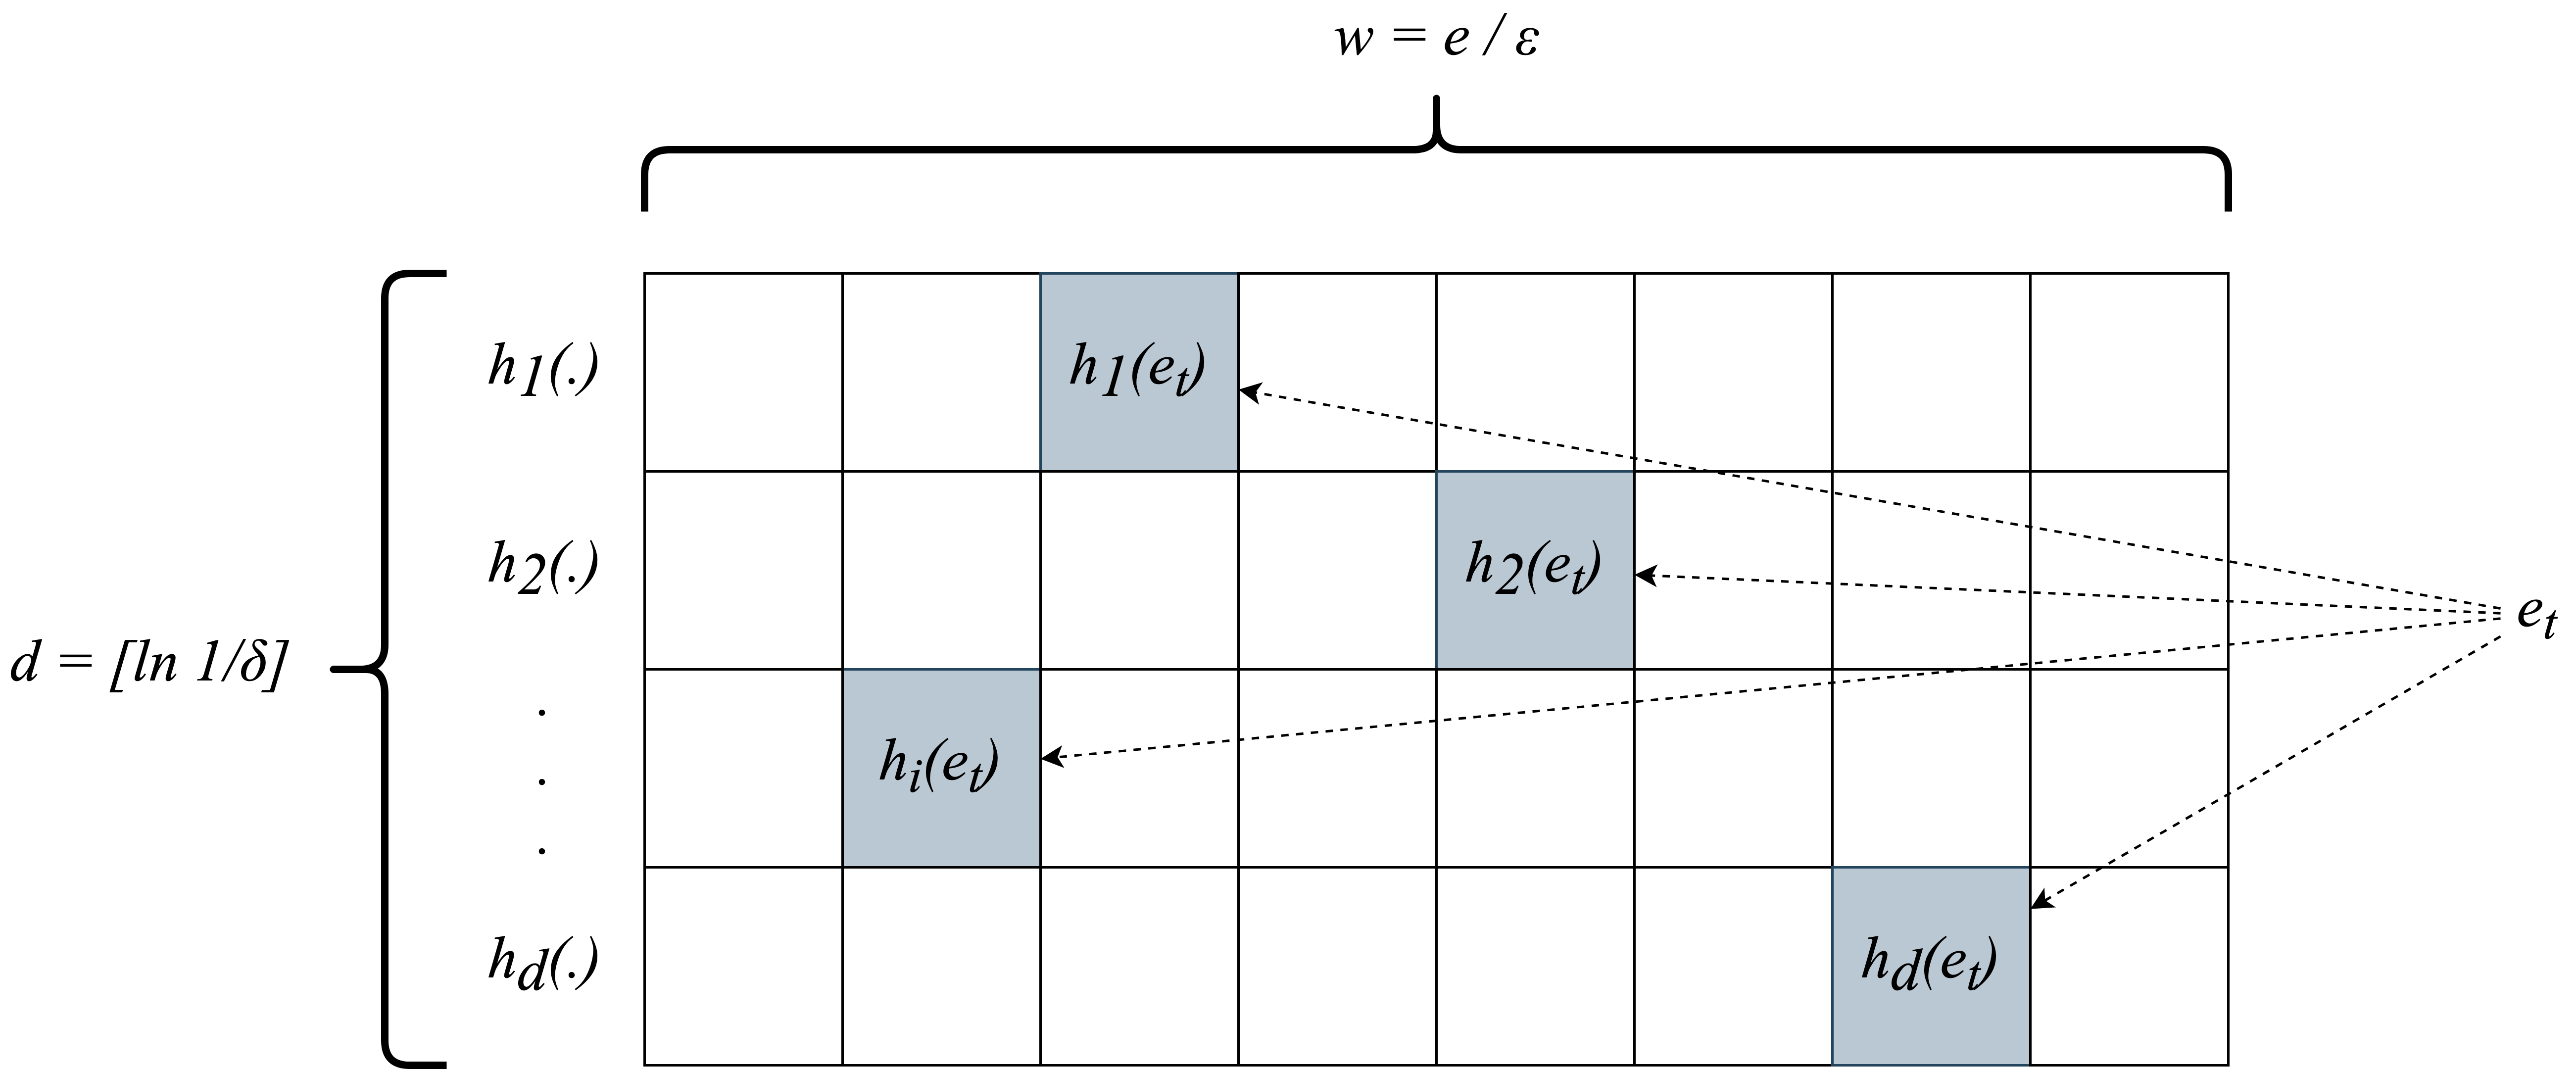
\includegraphics[width=0.9\textwidth]{images/countmin}
    \caption{CountMin sketch}
    \label{figure:countmin}
\end{figure}

\paragraph{}
CountMin\cite{cormode_improved_2003} could be considered as the pioneering work in summarizing data streams which are directly related to our research. CountMin\cite{cormode_improved_2003} is a data structure that is used for frequency approximation queries. The underlying idea behind the CountMin\cite{cormode_improved_2003} data structure is to hash the aggregated frequencies of the edges using multiple hash functions into predefined blocks as indicated in Figure \ref{figure:countmin}. A fixed sized will be stated at the time of creation of the CountMin\cite{cormode_improved_2003} sketch and irrespective of the volume of data stored, the size of the sketch does not have to be changed. The major drawback in following this procedure is that the error of the queries reduce as more and more data is introduced to the sketch. However despite these weaknesses, CountMin\cite{cormode_improved_2003} can be considered as a good generalized sketch at the time as many other sketches described in the literature are good for one single pre-specified aggregate computation. Therefore CountMin\cite{cormode_improved_2003} approach is not restricted to streaming graphs but other applications as well\cite{cormode_improved_2003}. 

\subsection{gSketch}

\paragraph{}
gSketch\cite{zhao_gsketch:_2011} is an extension of CountMin\cite{cormode_improved_2003} data structure. But unlike CountMin\cite{cormode_improved_2003} sketch, this is specifically geared towards summarizing graph streams. gSketch\cite{zhao_gsketch:_2011} is based on one of the two assumptions that,

\begin{enumerate}
    \item A graph stream sample is available.
    \item Both graph stream sample and a query workload sample are available.
\end{enumerate}

\begin{figure}[H]
    \centering
    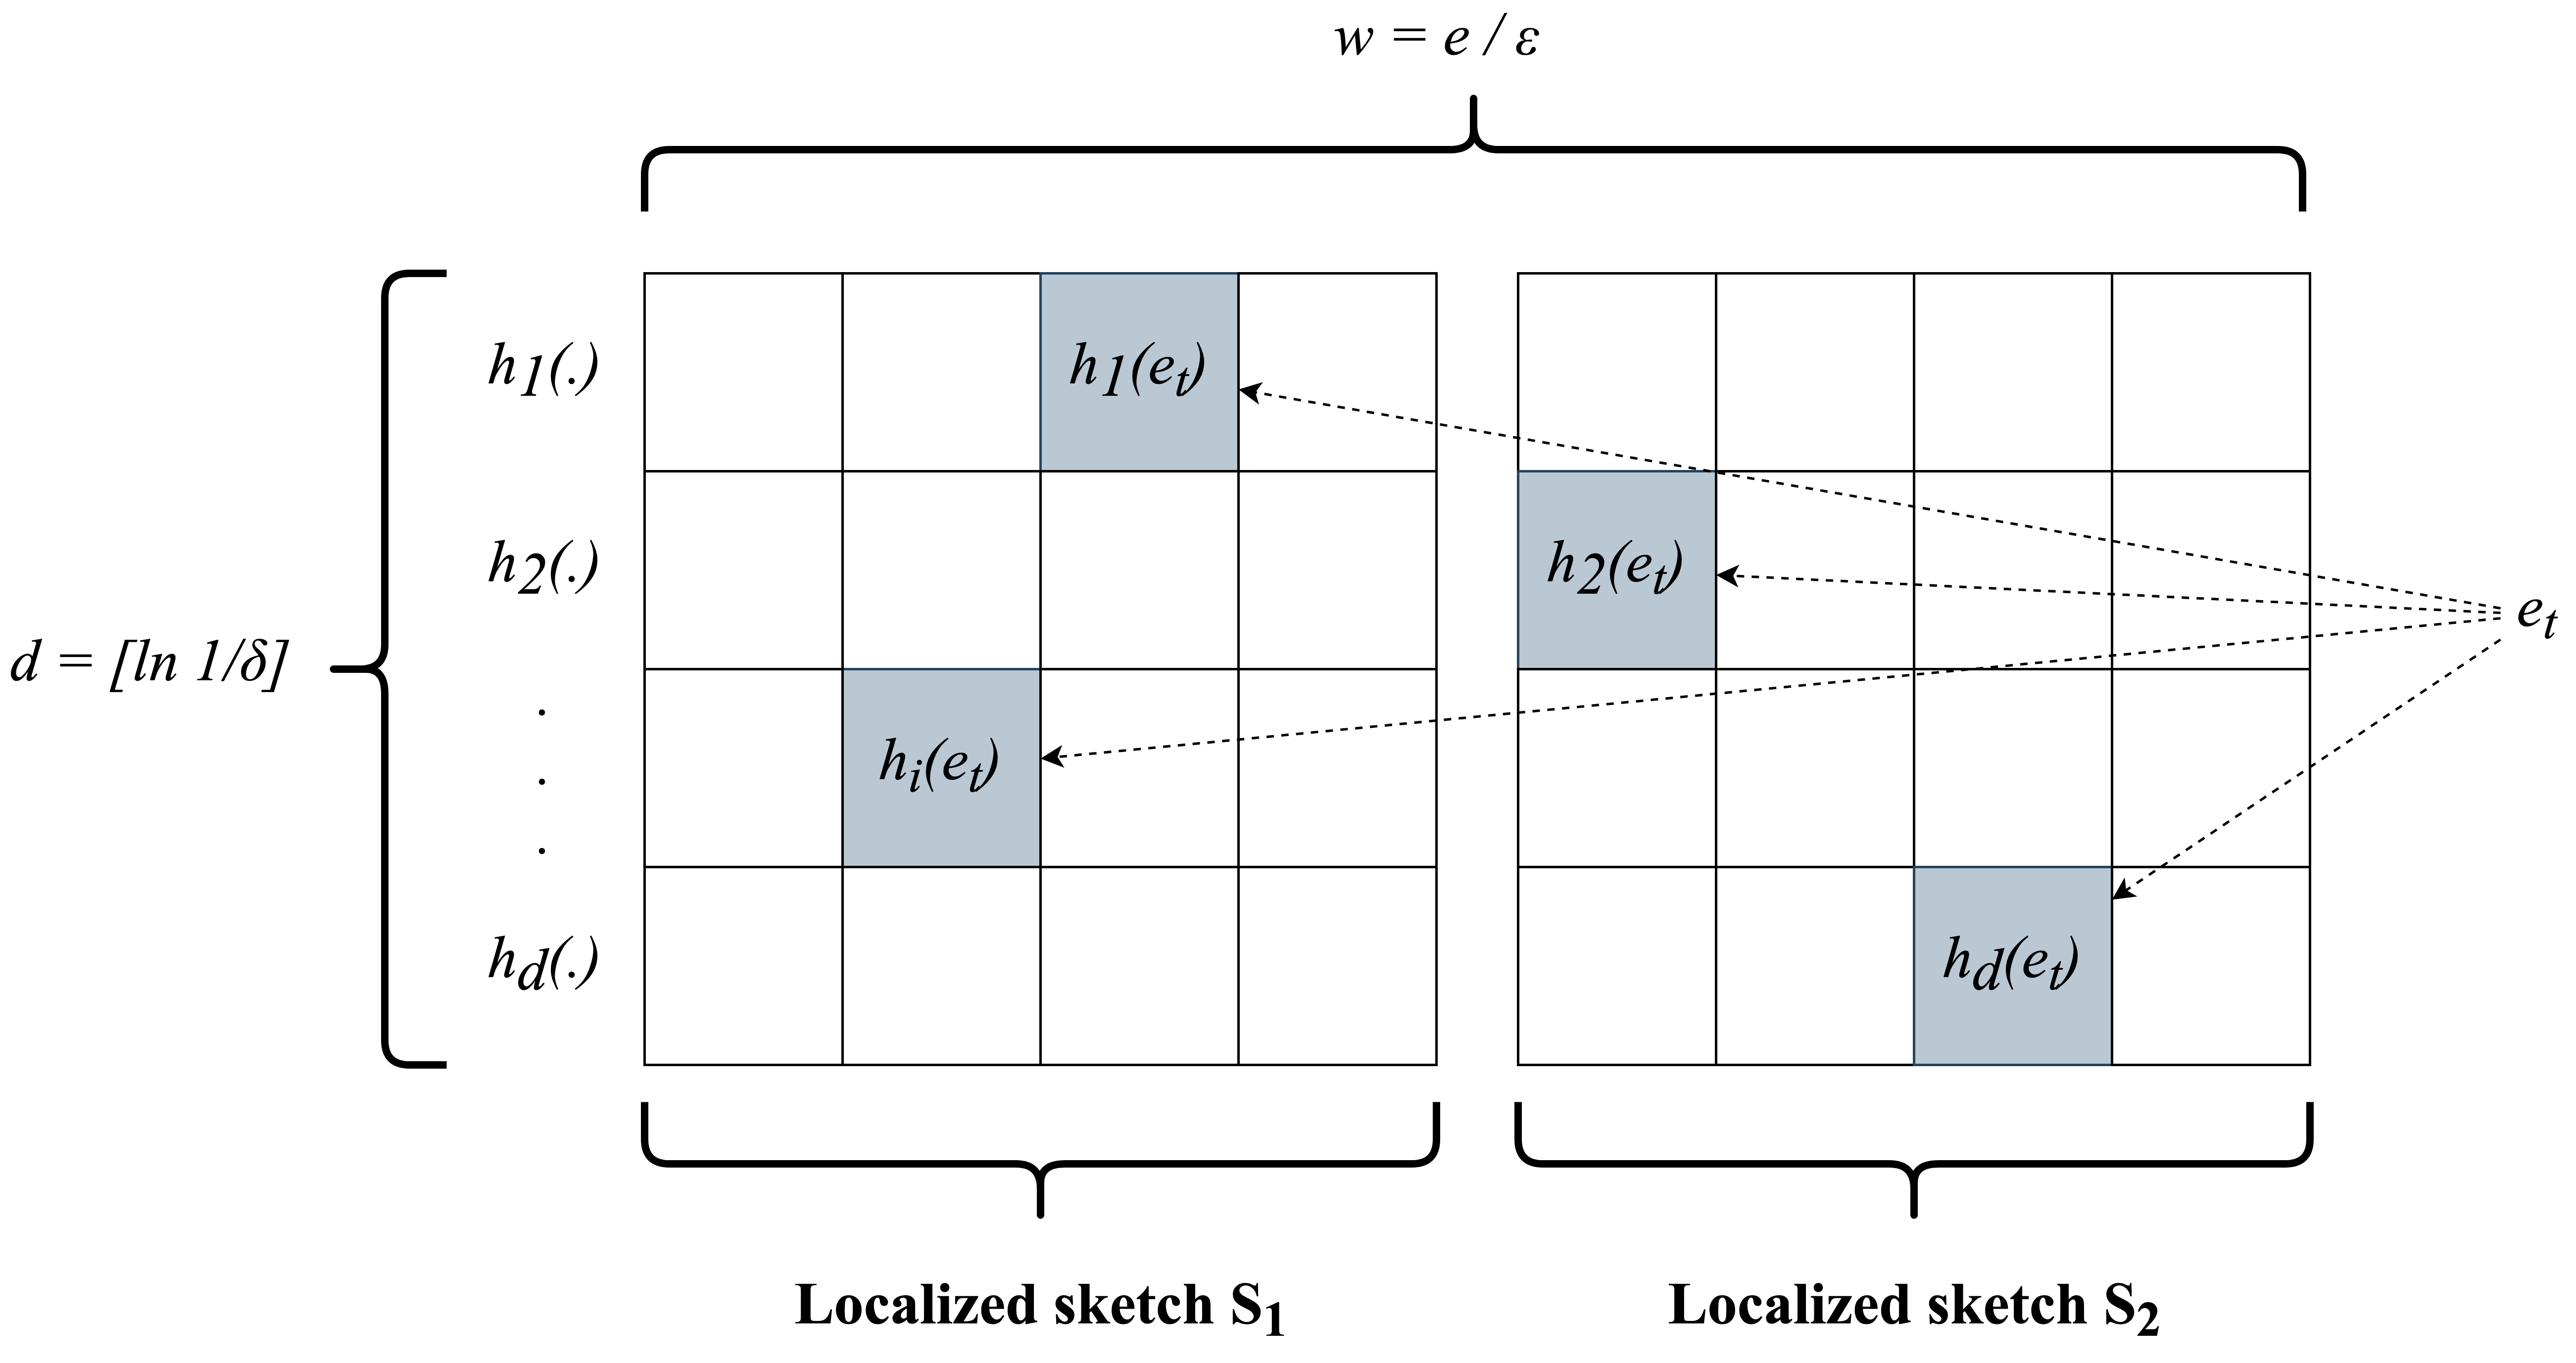
\includegraphics[width=0.9\textwidth]{images/gsketch}
    \caption{gSketch}
    \label{figure:gsketch}
\end{figure}

\paragraph{}
As per the previous sketching technique, CountMin\cite{cormode_improved_2003}, a global sketch is created for the entire graph stream. The disadvantage of this method is that any structural properties present in the graph stream are completely ignored throughout this process. gSketch\cite{zhao_gsketch:_2011} tries to avoid by considering the underlying structural properties of the graph. 

\paragraph{}
The specialty of gSketch\cite{zhao_gsketch:_2011} is to pre-process the stream samples and creating sketch partitions as indicated in Figure \ref{figure:gsketch}. Its goal is to maintain sufficient frequency uniformity within each localized sketch so that the query estimation can be optimized over the entire graph stream. 

\subsection{TCM}

\begin{figure}[H]
    \centering
    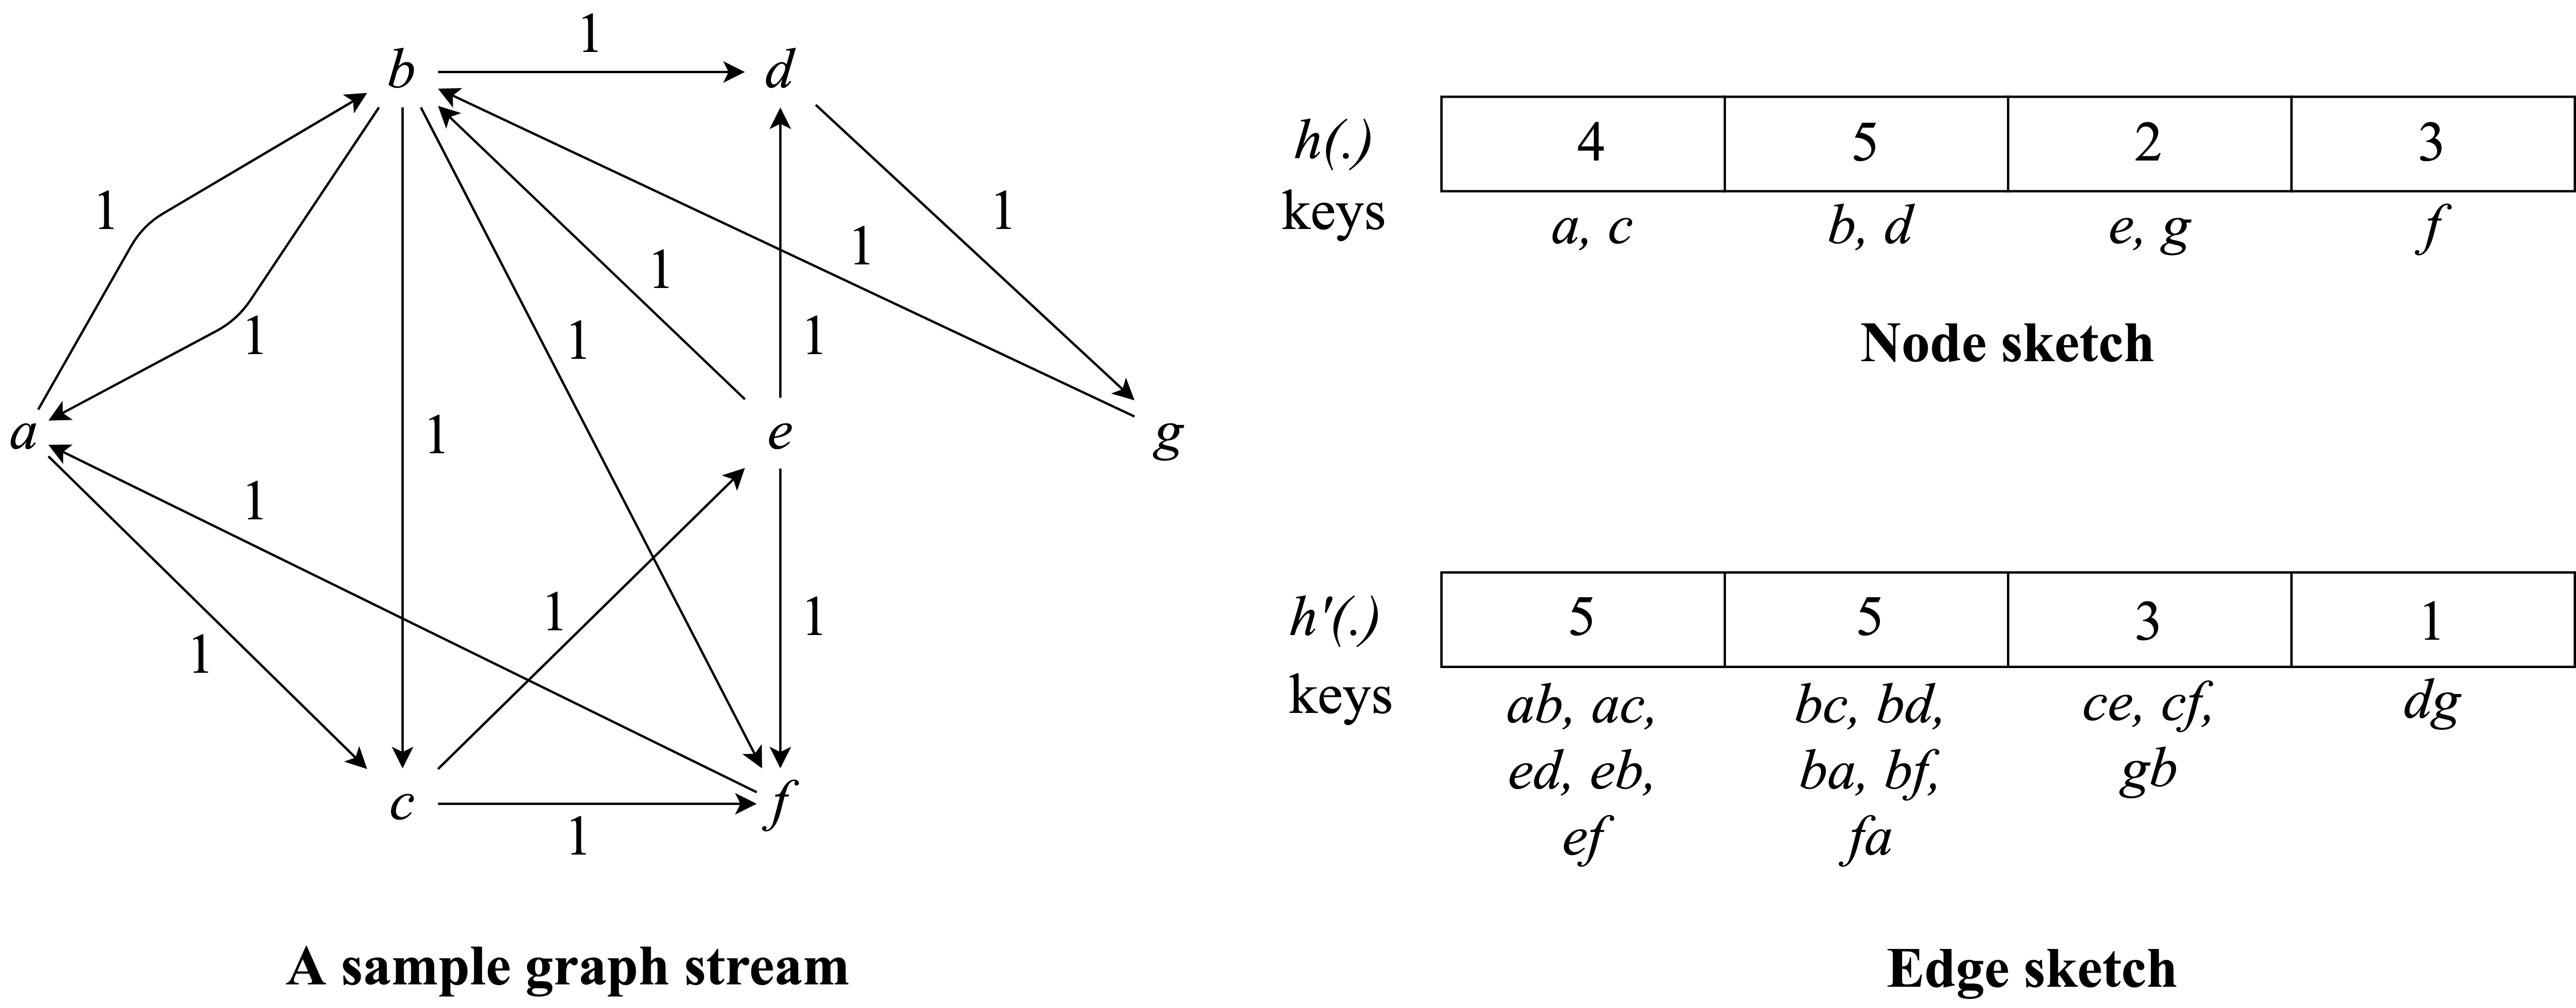
\includegraphics[width=\textwidth]{images/approximate_frequency_counts}
    \caption{Approximate Frequency Counts}
    \label{figure:afc}
\end{figure}

\paragraph{}
Approximate Frequency Count sketches store aggregated frequencies of edges in summarized form as shown in the example in Figure \ref{figure:afc}.

\paragraph{}
A disadvantage posed by all the approximate frequency count sketches like CountMin\cite{cormode_improved_2003} or gSketch\cite{zhao_gsketch:_2011} is that they do no store the locality of the nodes. Therefore they cannot be used for conditional node queries or queries involving node connectivity. If these queries were to be run, at least some of the information about the locality of nodes has to be retained in the graph synopses. TCM\cite{tang_graph_2016} can summarize both node and edge information in constant time. Because of that it can answer a wide range of queries unlike its predecessors. The structure of a TCM sketch is depicted in Figure \ref{figure:tcm}.

\begin{figure}[H]
    \centering
    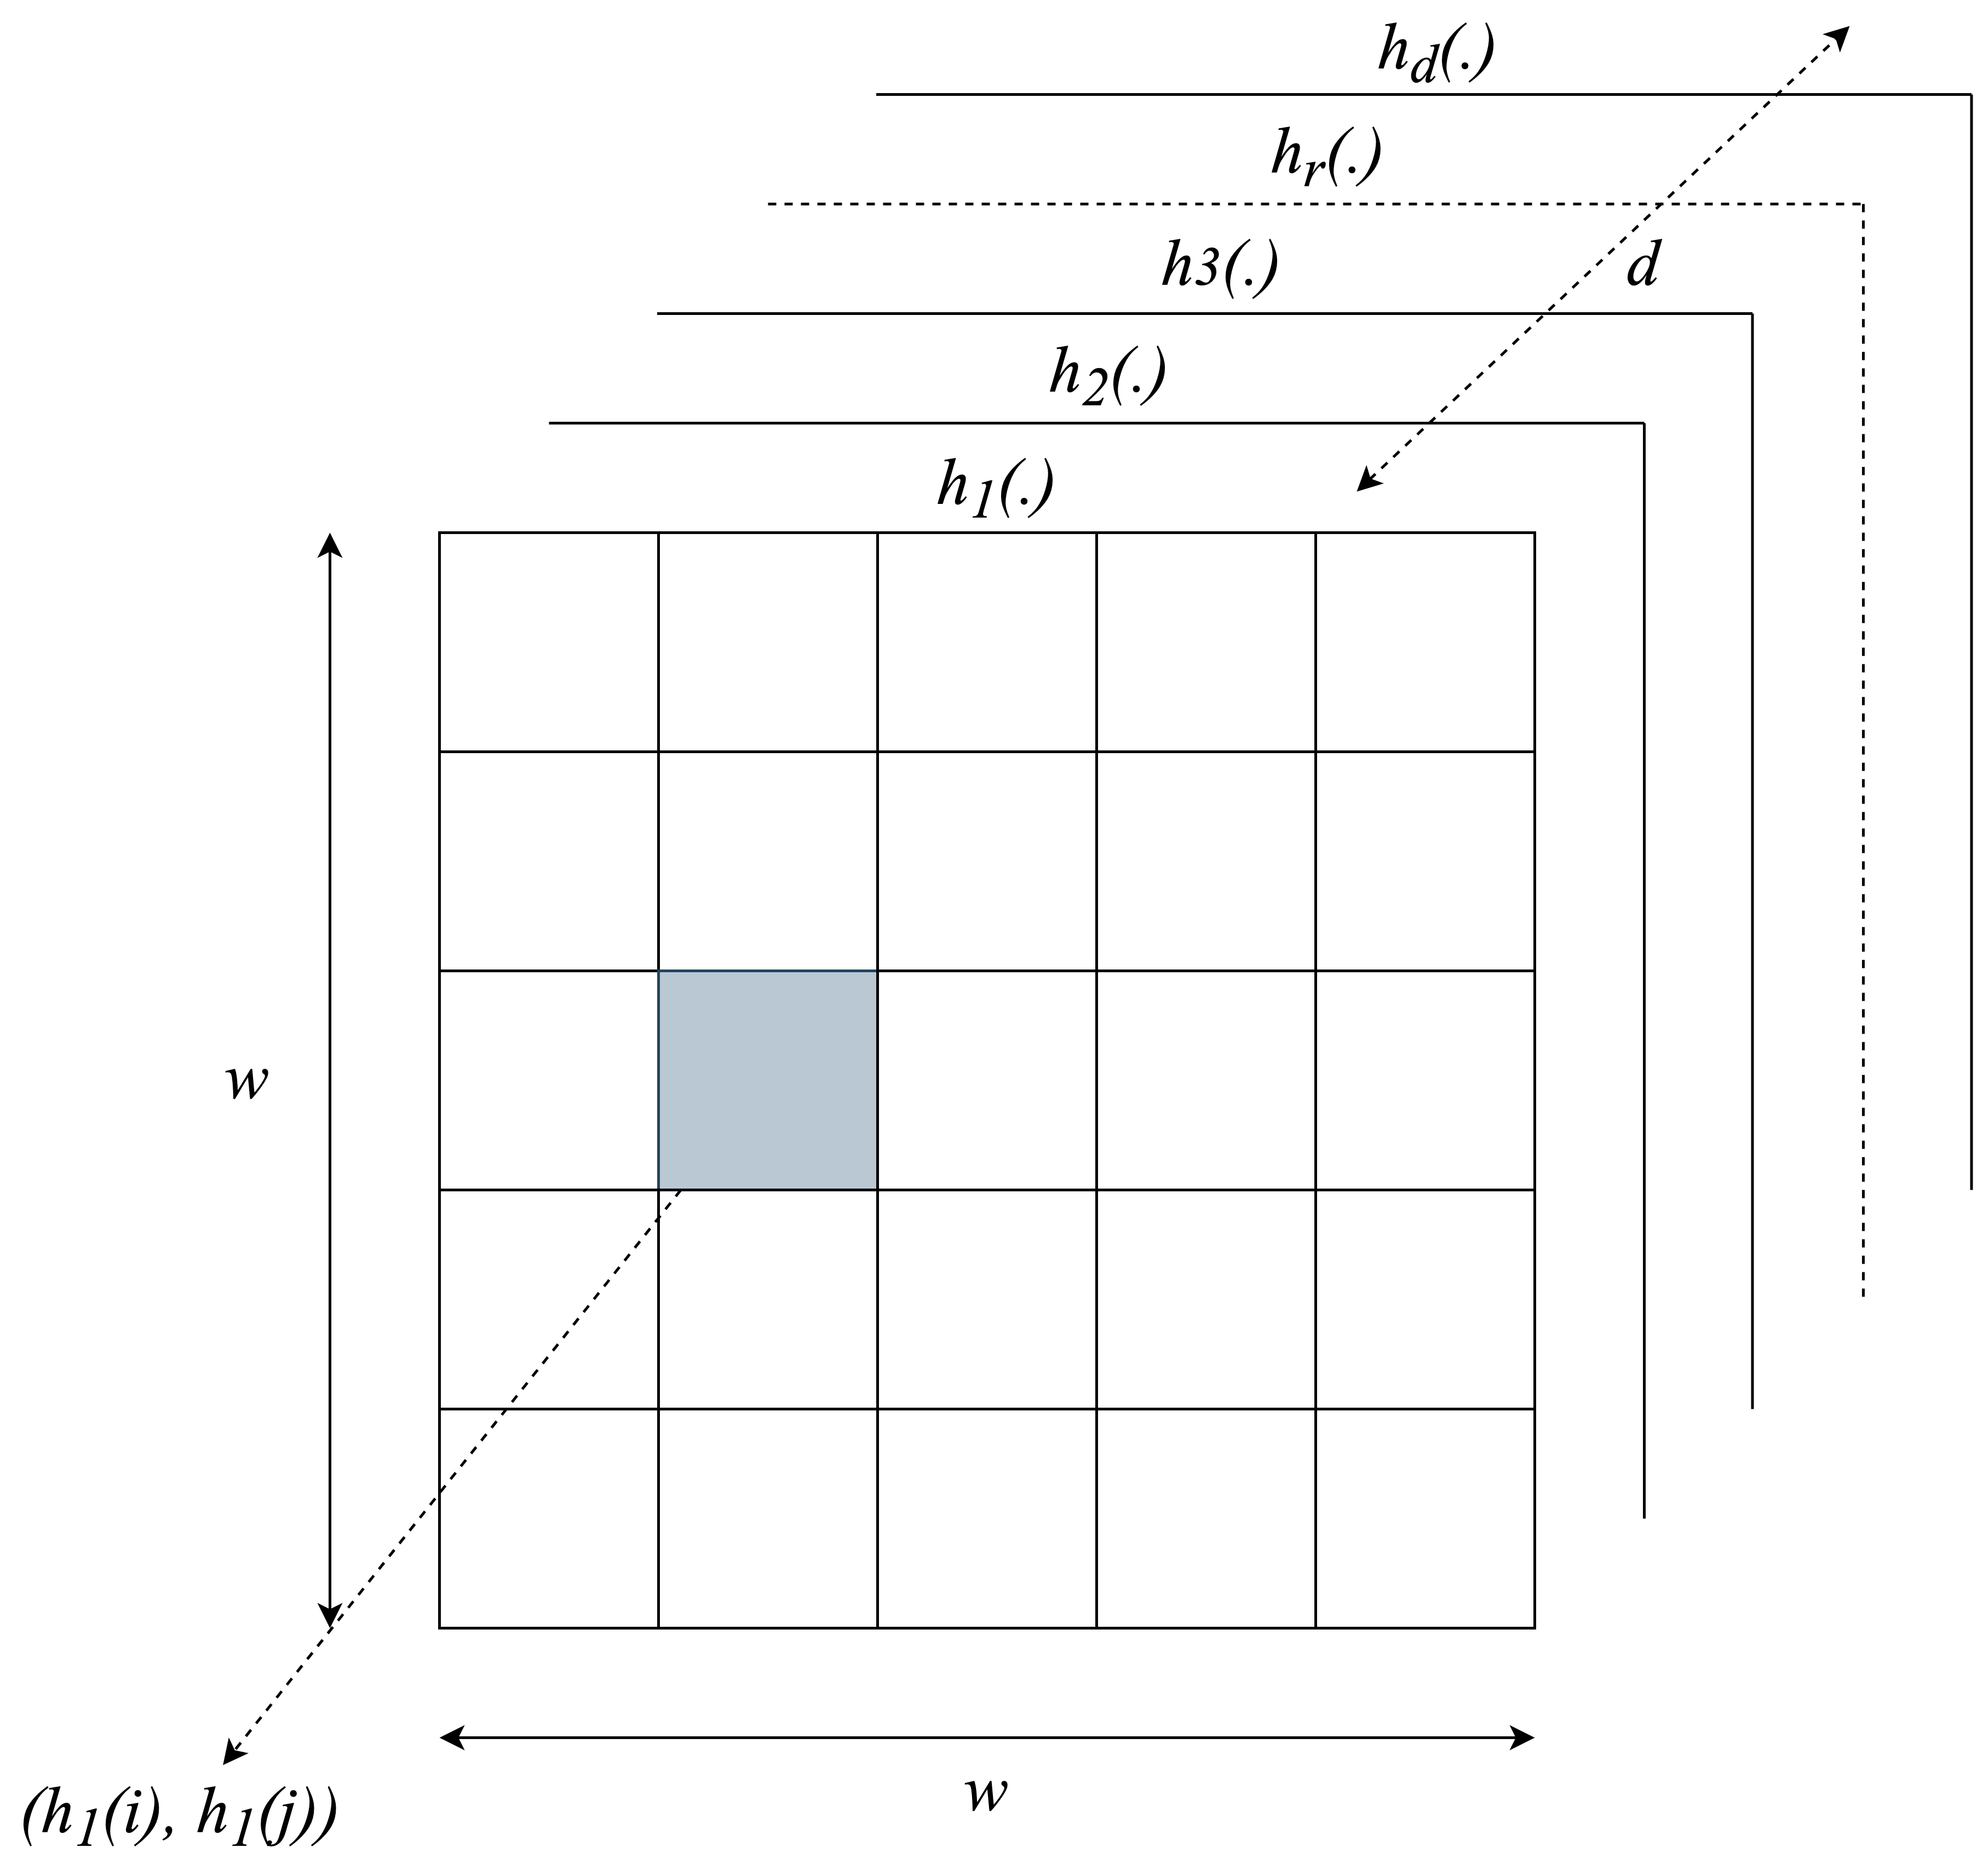
\includegraphics[width=0.5\textwidth]{images/tcm}
    \caption{TCM}
    \label{figure:tcm}
\end{figure}

\subsection{gMatrix}

\paragraph{}
gMatrix\cite{khan_query-friendly_2016} is a very similar to TCM and it was proposed in the same year as the TCM. However gMatrix\cite{khan_query-friendly_2016} paper consider about,

\begin{itemize}
    \item reverse hashing queries through pairwise independent hash functions;
    \item alternative options to extend sketch and space-saving synopses for achieving similar functionalities as gMatrix\cite{khan_query-friendly_2016};
\end{itemize}

which the TCM paper does not address. 

\subsection{GSS}

\paragraph{}
GSS\cite{gou_fast_2018} is the latest graph summarization technique that has been introduced up to date which was published in 2018. Even when using 1/256 memory size of the state of the art graph summarization algorithm, GSS\cite{gou_fast_2018} still significantly outperformed it for most queries\cite{gou_fast_2018}. The GSS paper\cite{gou_fast_2018} points out that even if TCM\cite{tang_graph_2016} and gMatrix\cite{khan_query-friendly_2016} supports all queries in the streaming graphs in contrast to CM sketches\cite{cormode_improved_2003} and gSketches\cite{zhao_gsketch:_2011} which only supports queries for edges and do not get involved with the topology of the underlying graph, they suffer from poor accuracy. GSS\cite{gou_fast_2018} improves upon TCM\cite{tang_graph_2016} and gMatrix\cite{khan_query-friendly_2016} to increase the accuracy with less memory usage. 

\paragraph{}
GSS\cite{gou_fast_2018} defines three graph primitives as,

\begin{itemize}
    \item Edge query 
    \item 1-hop Successor query 
    \item 1-hop Precursor query
\end{itemize}

By supporting all these 3 types of queries it is possible to reconstruct the entire graph. Therefore it is also possible to run any kind of query against a sketch which supports all 3 of the above primitives. 

\paragraph{}
The intuition behind the basic version of the GSS\cite{gou_fast_2018} can be illustrated as below. 

\begin{figure}[H]
    \centering
    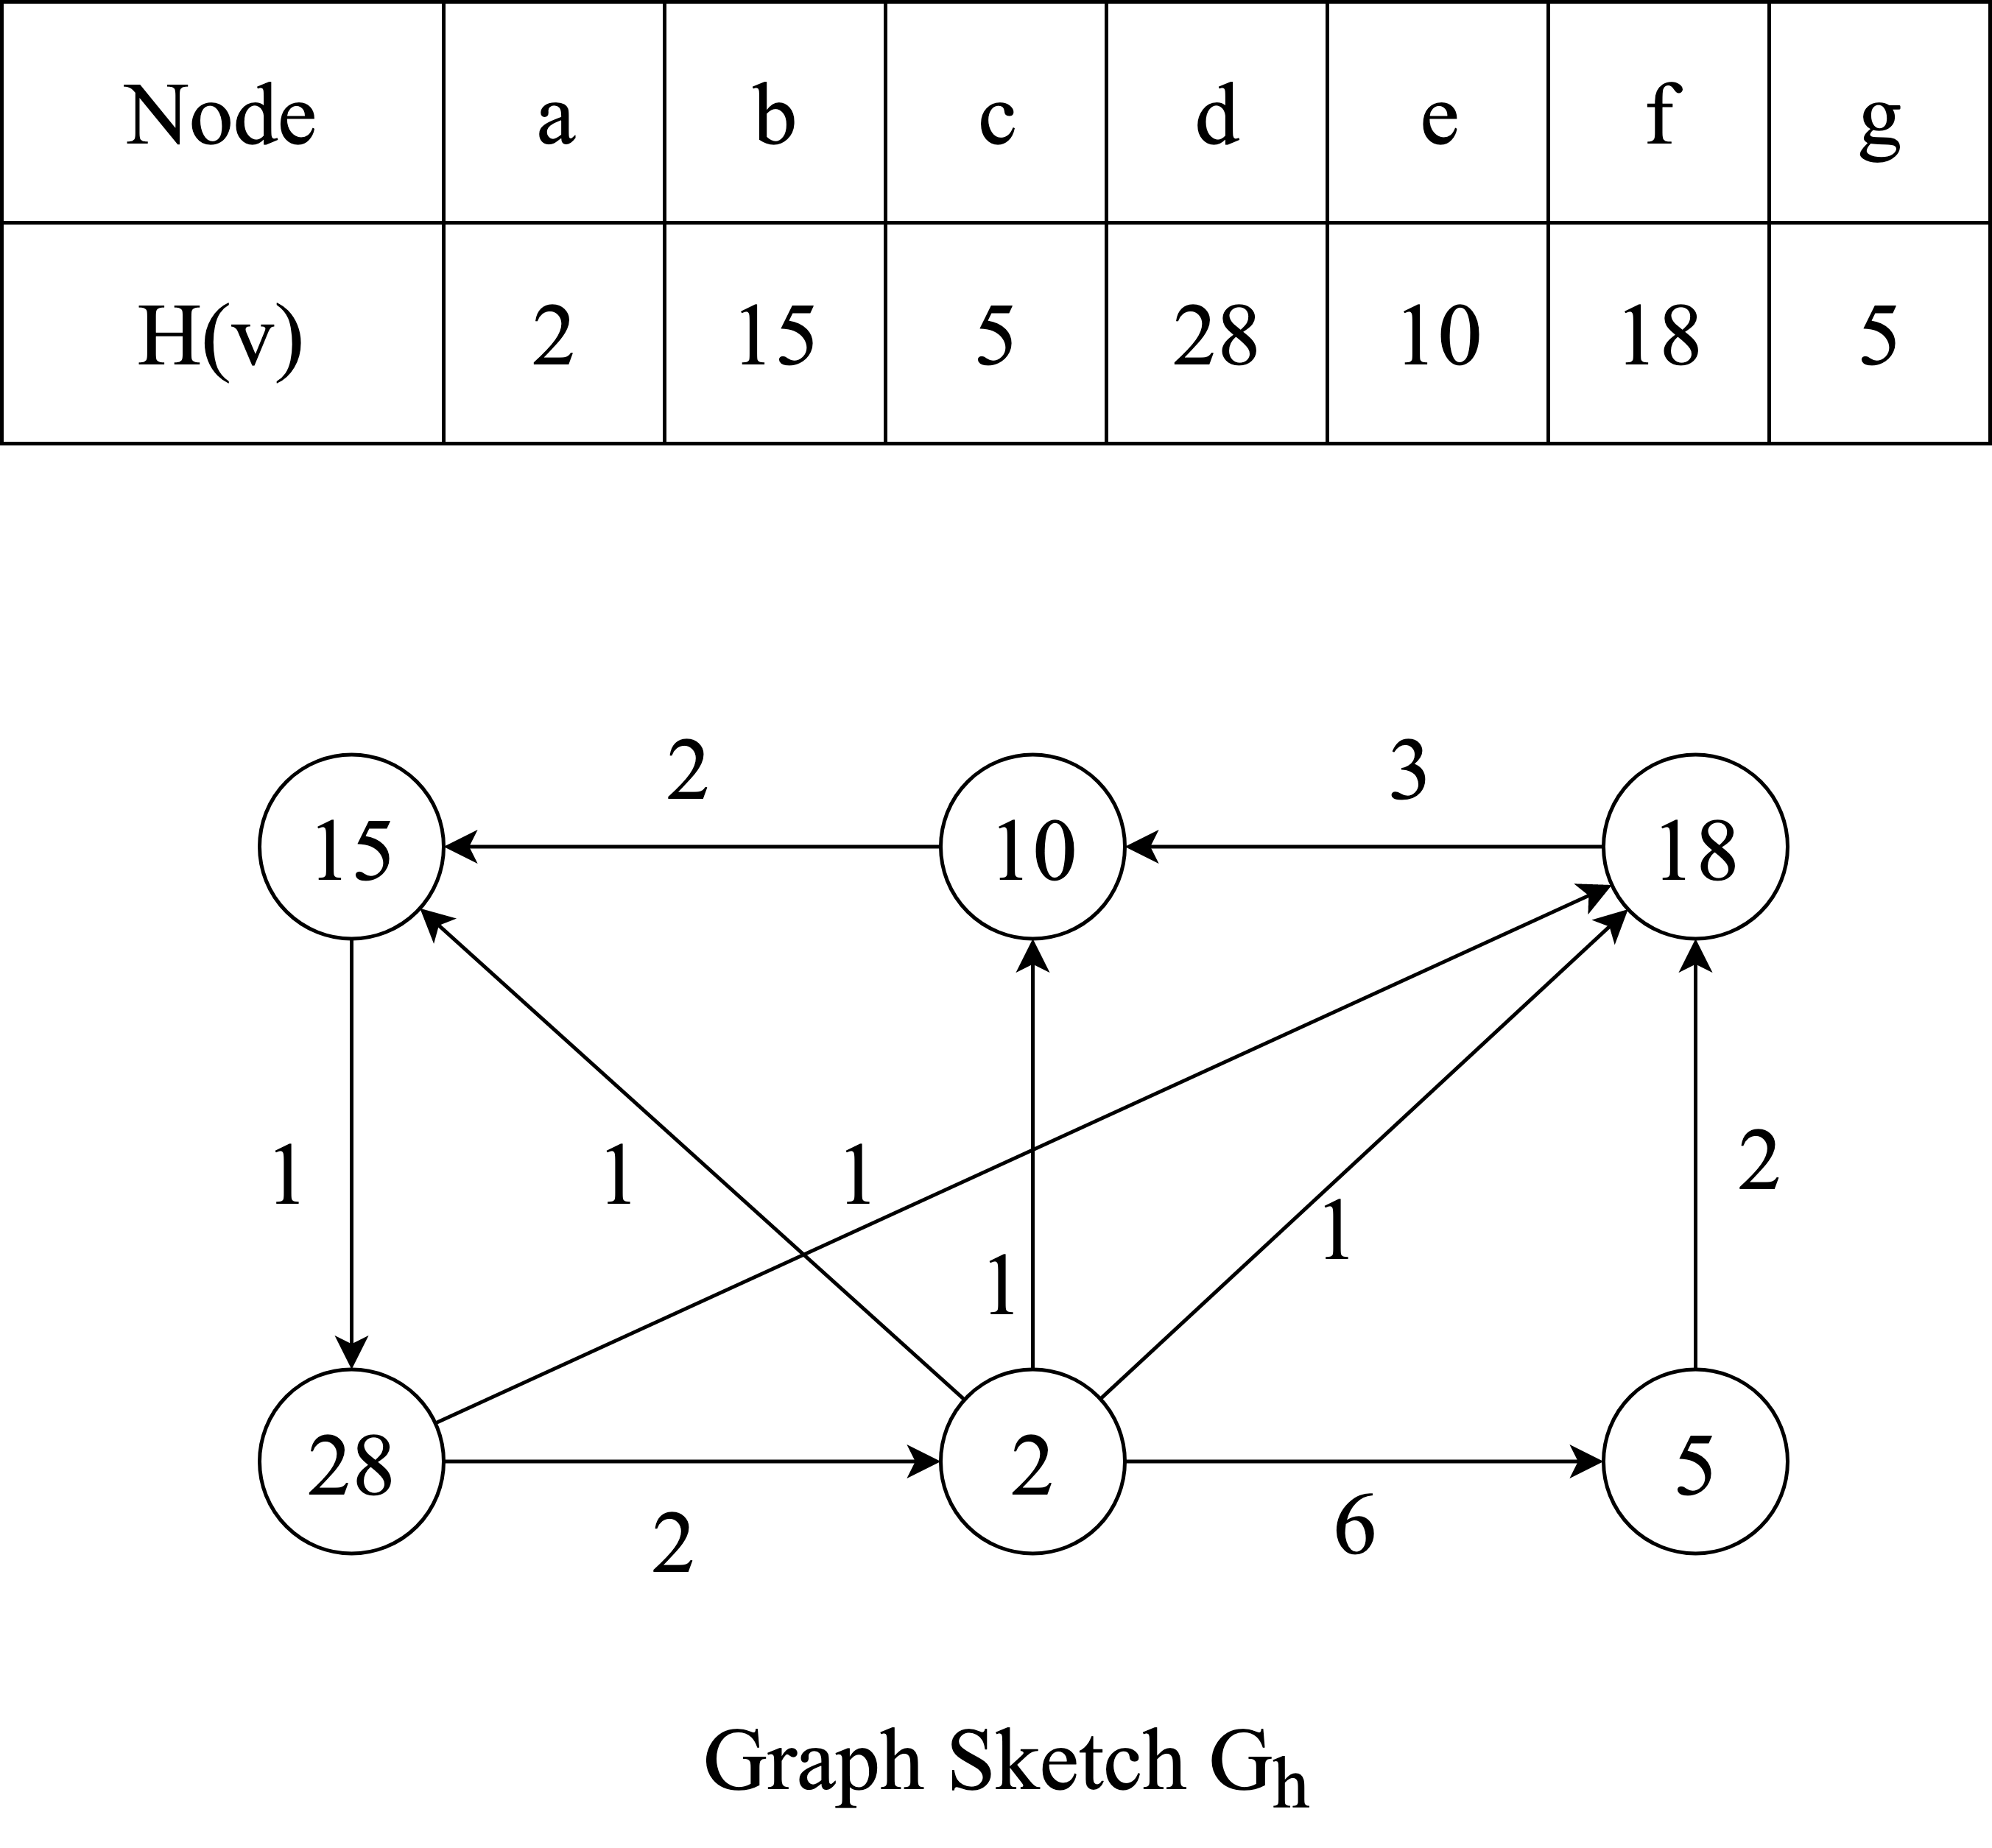
\includegraphics[width=0.5\textwidth]{images/gss1}
    \caption{A sample map function\cite{gou_fast_2018}}
    \label{figure:gss1}
\end{figure}

\paragraph{}
\(H(.)\) is a hash function which is used on the vertices of the original graph stream to create the graph sketch \(G\textsubscript{h}\) as indicated in Figure \ref{figure:gss1}.

\paragraph{}
A GSS\cite{gou_fast_2018} sketch consists of two parts, 

\begin{itemize}
    \item An \(m \times m\) adjacency matrix
    \item List buffer B for leftover edges
\end{itemize}

\paragraph{}
For each node in the sketch graph \(G\textsubscript{h}\), an address \(h(v)\) and a fingerprint \(f(v)\) is defined. Each edge \(H(s)\), \(H(d)\) is mapped into a bucket in the row \(h(s)\), column \(h(d)\) of the matrix. \([\langle f(s), f(d)\rangle, w]\) is recorded in the corresponding bucket of the matrix, where \(w\) is the edge weight and \(f(s)\), \(f(d)\) are the fingerprints for the source and destination. This can be seen in the sample of GSS sketch shown in Figure \ref{figure:gss2}.

\begin{figure}[H]
    \centering
    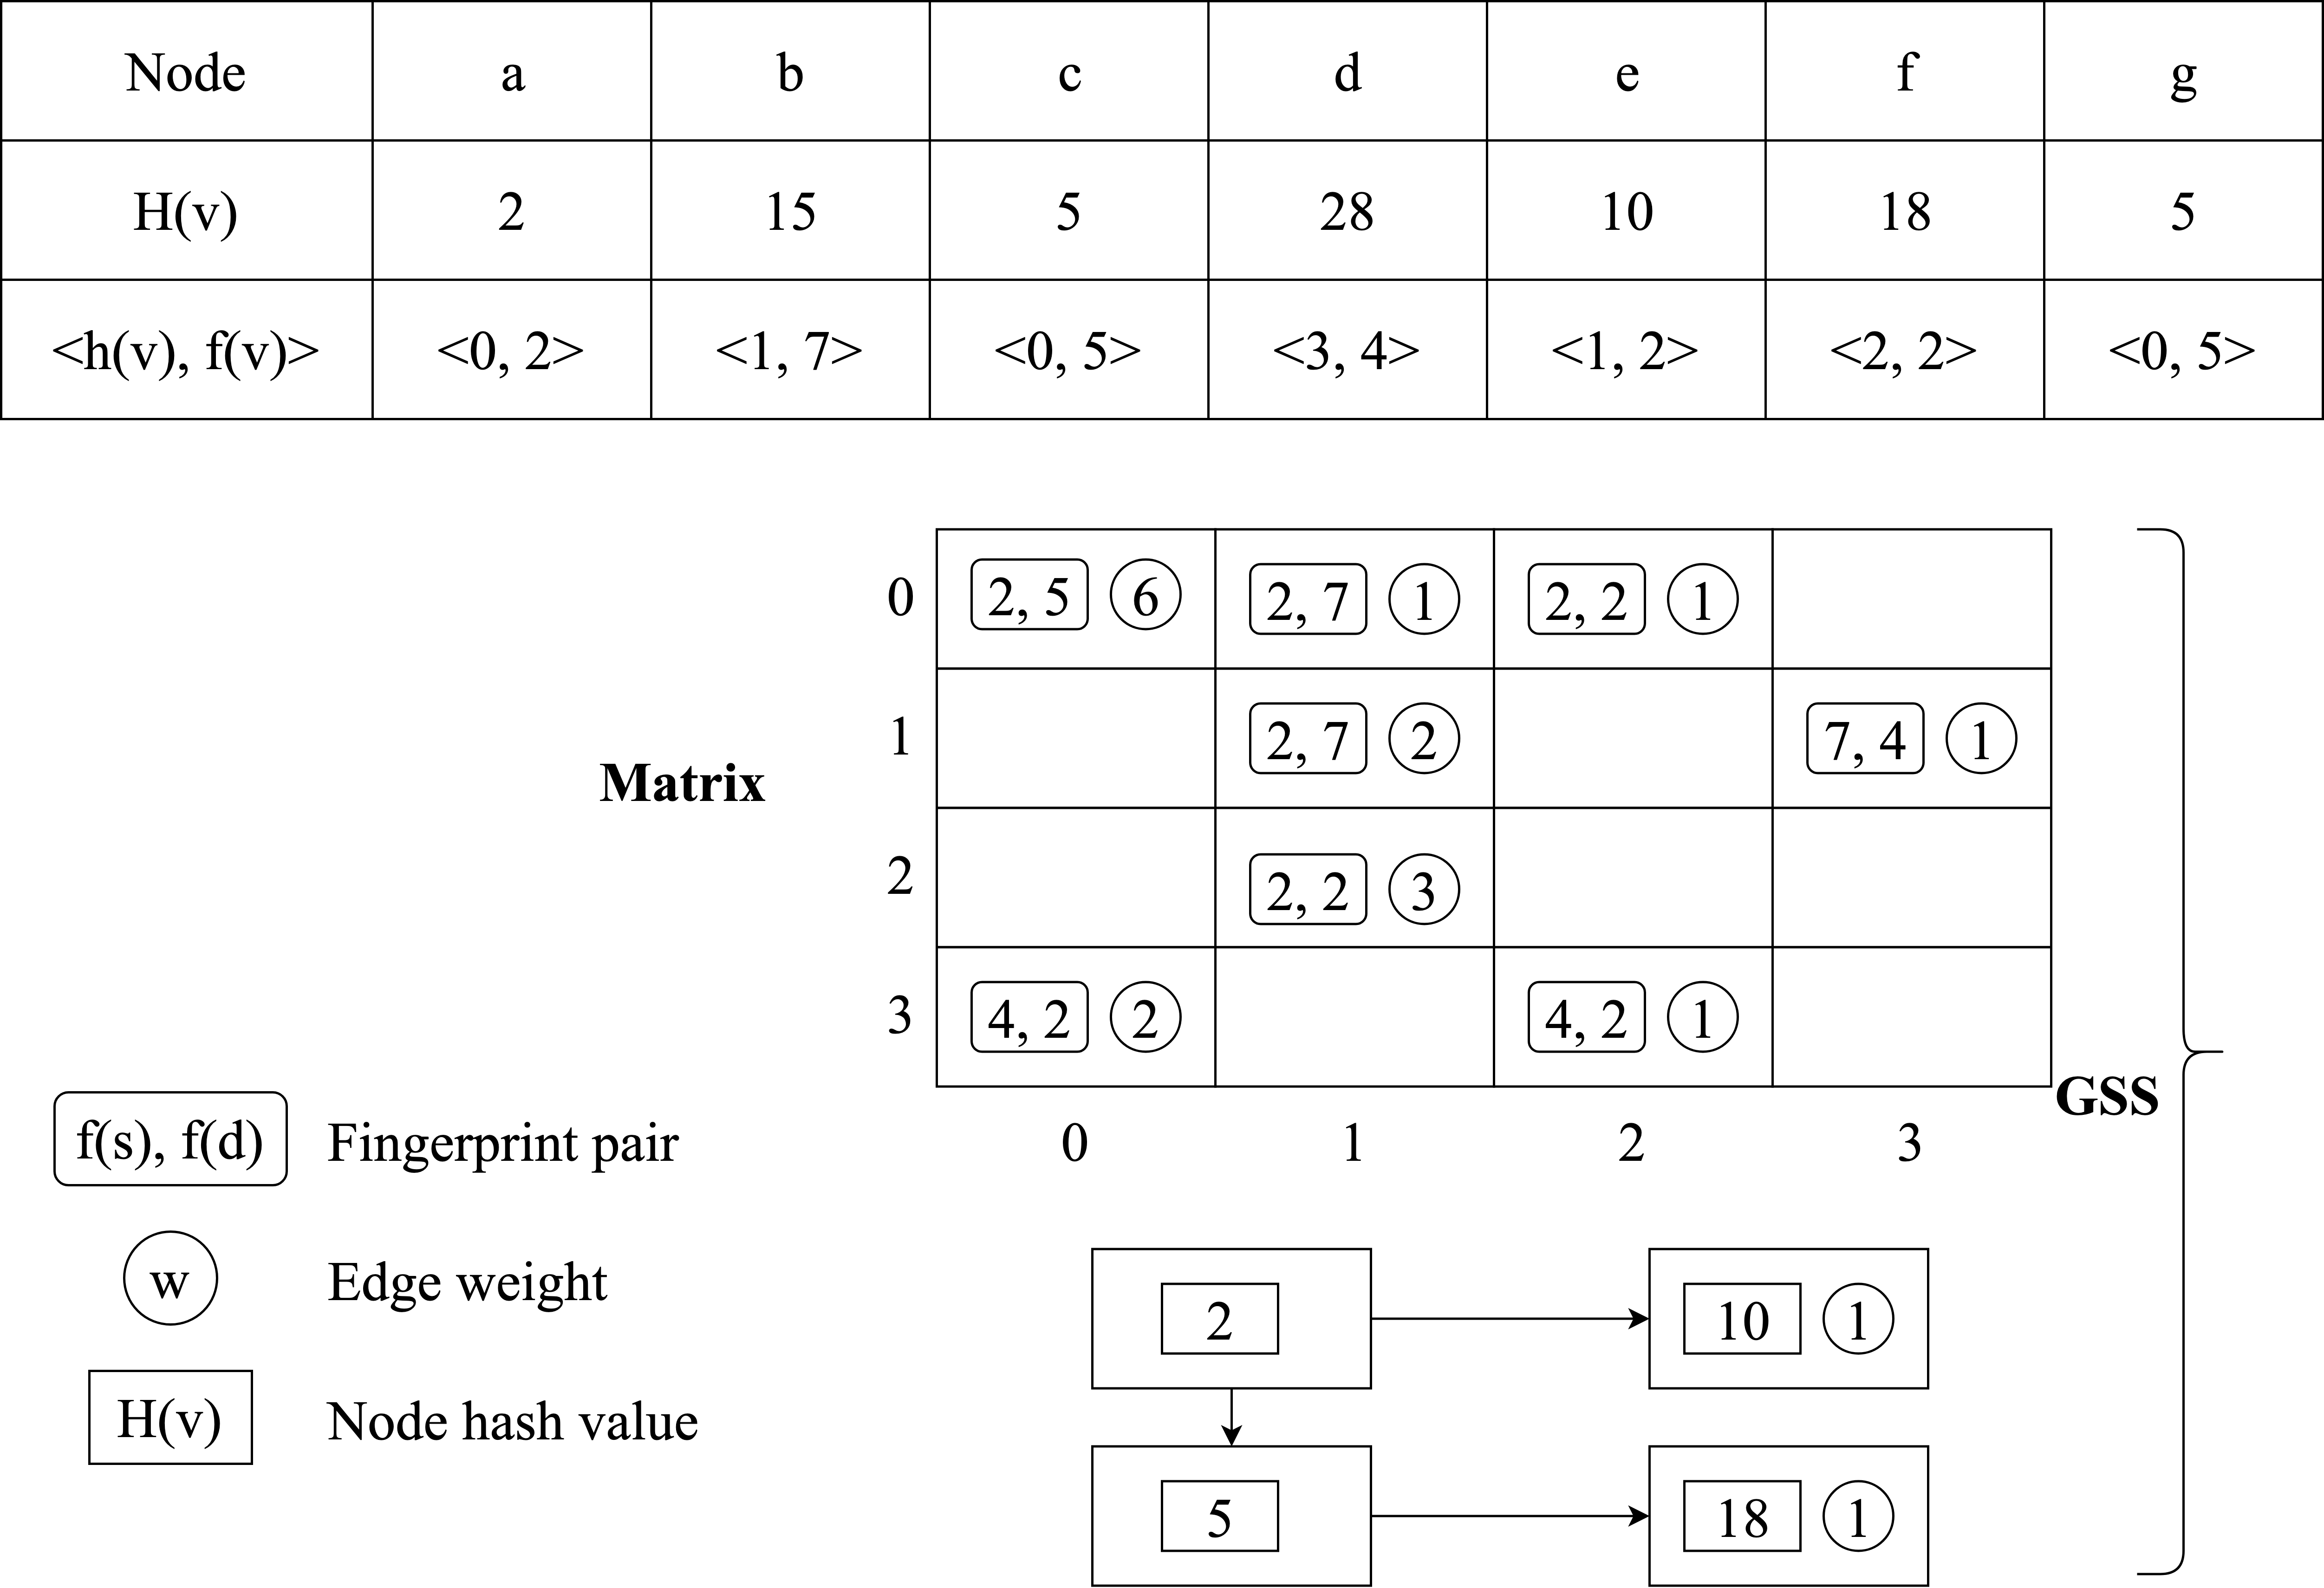
\includegraphics[width=0.9\textwidth]{images/gss2}
    \caption{A sample version of the basic data structure\cite{gou_fast_2018}}
    \label{figure:gss2}
\end{figure}

% \section{Summary}

% \paragraph{}
% Some summary----